\chapter{General Description of the Project}
\label{chap:general-description}

\section*{Introduction}

This chapter introduces the host company and the context of the project. The existing
problems are detailed to define the specifications and clarify the requested work. We then
present the theoretical foundations relevant to the project and explain the adopted work
methodology.

\section{Host company}
\label{sec:host-company}

This section provides an overview of STMicroelectronics, its history, the ST Tunis site,
and the technically oriented marketing and application support team in which this project
was carried out.

\subsection{Presentation}

STMicroelectronics is a global semiconductor company dedicated to enhancing people's lives
through innovative electronic solutions~\cite{st-about}. With one of the most extensive
product portfolios in the industry, ST serves over 200,000 customers worldwide, achieving
net revenues of \$13.27~billion in 2024~\cite{st-investors}.

The company was established in June 1987 as SGS-THOMSON Microelectronics, following the
merger of SGS Microelettronica (Italy) and Thomson Semiconductors (France). The name
``STMicroelectronics'' was officially adopted in May 1998. Figure~\ref{fig:st-logo}
shows the company's official logo.

\begin{figure}[H]
\centering

\includegraphics[width=0.35\textwidth]{Logos/STMicroelectronics.png}
\caption{STMicroelectronics logo.}
\label{fig:st-logo}
\end{figure}

With more than 80 sales and marketing offices and 14 primary manufacturing locations
across the globe, the corporation employs over 50,000 people~\cite{st-about}.

\subsection{STMicroelectronics vision and markets}

STMicroelectronics has prioritised technological innovation in its strategy for over
25~years. It makes market-driven investments in technology development with the goal of
commercialising cutting-edge innovations that create immediate value for its customers
~\cite{st-strategy}. Today, with a robust pipeline, ST delivers products that are smaller,
faster, more energy-efficient, and equipped with new features. Driven by a global lean
manufacturing culture, ST addresses three main end markets: automotive, industrial, and
personal electronics --- and offers engagement models ranging from application-specific
embedded systems to application-specific standard products.

\subsection{STMicroelectronics Tunis}

The ST Tunis site, located in Technopark El~Ghazela, began operations in 2001 with nine
engineers. Today it has expanded to more than 200~employees working across design, tools,
applications, quality, and support functions~\cite{st-about}. The facility participates in
every stage from the initial design of new circuits to the final verification of their
functionality before mass production.

The Microcontroller Division (MCD) is dedicated to the design of microcontrollers,
demonstration platforms, and solutions for consumer use. It is responsible for the
development of drivers and embedded software --- specifically the validation and
development of libraries and firmware that drive ST microcontrollers.
Figure~\ref{fig:st-site-org} shows the organisational structure of the MCD division at the
Tunis site; the Maintenance team, highlighted, is where this project was carried out.

\begin{figure}[H]
\centering
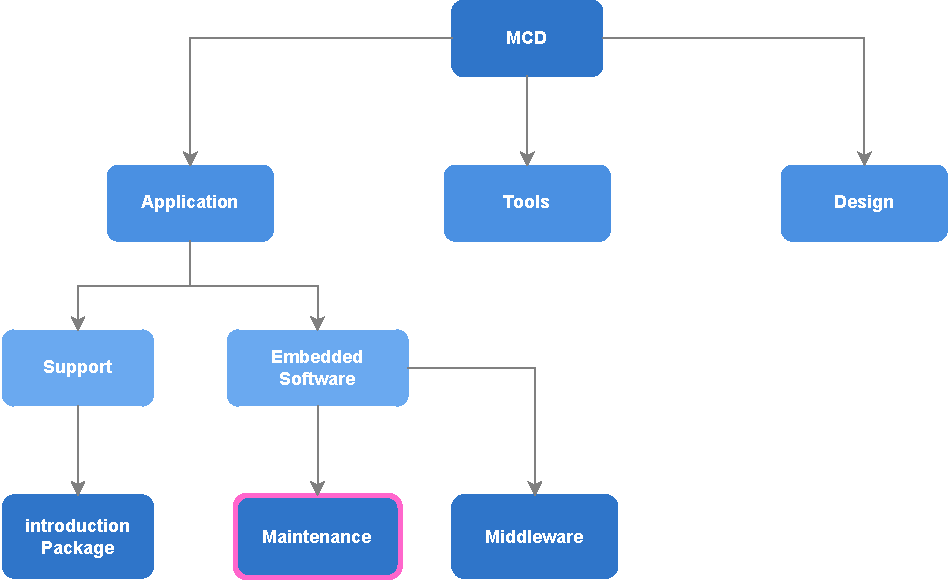
\includegraphics[width=0.7\textwidth]{Figures/chapter1/st-site-organization.pdf}
\caption{Organisational structure of the Microcontroller Division (MCD) at ST Tunis.
The Maintenance team (highlighted) is the host team of this project.}
\label{fig:st-site-org}
\end{figure}

This project was carried out in the \textbf{Technical Marketing and Application Support}
team under MCD. This team includes two sub-teams:

\begin{itemize}
\item \textbf{The GitHub team}: supports customers via GitHub, publishes updates of HAL
drivers, and maintains example projects to facilitate application development based on
STM32 microcontrollers.
\item \textbf{The Maintenance and Validation team}: ensures customer satisfaction through
bug maintenance and functional validation of manufactured microcontrollers and their
associated HAL versions. This team represents the junction linking software and hardware
design processes to implementation and industrialisation.
\end{itemize}

\section{Project presentation}
\label{sec:project-presentation}

\subsection{Project framework}

As part of our training in Computer Engineering at the Faculty of Sciences of Tunis (FST),
University of Tunis El~Manar (UTM), we conclude our education with an end-of-studies
project (PFE). In this context, our project --- entitled \emph{STM32Cube Competitor
Benchmark} --- took place within STMicroelectronics Tunis over a period of six months
(February--September 2026).

\subsection{Project context}
\label{sec:project-context}

The embedded microcontroller market is highly competitive. When an engineer evaluates an MCU
for a new design, the choice between STMicroelectronics and competing vendors (GigaDevice
GD32, NXP, Texas Instruments, Renesas) often depends on measurable differences: firmware
footprint, execution speed, middleware maturity, and development-tool productivity. The
technical marketing team at ST needs objective, reproducible data that quantifies where the
STM32Cube ecosystem outperforms its competitors, where gaps exist, and what concrete
enhancements would close those gaps.

At the start of this project, no systematic benchmarking methodology existed within the
team. Cross-vendor comparisons were ad-hoc, performed manually on a case-by-case basis,
and difficult to reproduce or communicate convincingly to stakeholders.

\subsection{Problematic}
\label{sec:problematic}

Producing actionable competitive intelligence for the marketing team requires answering
precise questions: for a given software stack (e.g.\ USB device, FreeRTOS integration),
running identical scenarios on ST and on a competitor, how do the two platforms compare in
flash and RAM footprint, execution performance, and middleware completeness? And where ST
lags, what specific enhancements --- at the HAL, middleware, or configuration level ---
would close the gap?

Answering these questions rigorously raises several challenges:

\begin{enumerate}
\item \textbf{Scenario design}: each benchmark must exercise the same functionality on both
platforms under identical, well-defined conditions so that the comparison is fair and the
results are meaningful.
\item \textbf{Porting fidelity}: reproducing an STM32 reference scenario on a competitor
requires preserving exact runtime semantics --- task structure, timing, synchronisation,
reporting format --- to avoid comparing apples to oranges.
\item \textbf{Result extraction and interpretation}: raw numbers (kilobytes, cycles,
milliseconds) must be attributed to comparable architectural layers and interpreted in
terms of engineering trade-offs, not merely listed.
\item \textbf{Scale and reproducibility}: the team needs to cover multiple vendors and
multiple stacks with consistent methodology, so that results are comparable across
campaigns and over time.
\end{enumerate}

\subsection{Proposed solution}
\label{sec:proposed-solution}

Our solution is a structured benchmarking methodology centred on three deliverables:

\begin{enumerate}
\item \textbf{Benchmark scenarios}: for each software stack under evaluation (USB device
stack, FreeRTOS, etc.), we design a set of concrete, reproducible scenarios that both the
STM32 reference and the competing platform must run identically. Each scenario exercises a
specific aspect of the stack (e.g.\ HID, CDC, and MSC for USB device).
\item \textbf{Comparative results and interpretation}: for each scenario, we extract
per-layer footprint figures, execution metrics, and qualitative observations, then
interpret them to show where ST is stronger, where the competitor leads, and why.
\item \textbf{Enhancement proposals}: where the data reveals a gap unfavourable to ST, we
identify the root cause and propose targeted improvements --- whether at the HAL driver
level, in middleware configuration, or in linker/startup overhead.
\end{enumerate}

To support this workflow at scale and ensure reproducibility, we developed two supportive
tools in parallel:

\begin{itemize}
\item \textbf{MCU Workflow Studio} --- a cross-vendor firmware footprint analysis
application that automates linker-map comparison, layer classification, and result export
(detailed in Chapter~2).
\item \textbf{MCU Benchmark Copilot Agent} --- a custom AI agent system that accelerates
benchmark creation, porting, and debugging while enforcing fairness and semantic
equivalence (detailed in Chapter~3).
\end{itemize}

These tools are parallel engineering contributions that enhance the benchmarking effort;
they are not the benchmarks themselves. The core deliverable remains the benchmark results
and the enhancement proposals they yield.

\subsection{Mission and objectives}
\label{sec:objectives}

The mission of this internship is to provide the STMicroelectronics technical marketing
team with rigorous, reproducible, and interpretable competitive benchmark data. Specifically,
the project aims to:

\begin{enumerate}
\item Design benchmark scenarios for selected software stacks, ensuring fairness and
semantic equivalence between ST and each competitor.
\item Execute the benchmarks on representative hardware, extracting flash/RAM footprint,
execution performance, and qualitative observations per scenario.
\item Compare and interpret the results layer by layer, highlighting where ST excels and
where gaps exist.
\item Formulate concrete enhancement proposals for STM32Cube where the data reveals room
for improvement.
\item Develop supportive tools (footprint analyser, benchmark agent) to make the
methodology reproducible and scalable beyond this project.
\end{enumerate}

\section{Theoretical foundations}
\label{sec:theory}

This section presents the background concepts essential for understanding the technical
aspects of the project: the STM32 microcontroller ecosystem, firmware memory footprint, and
the linker-map artefact that our tools consume.

\subsection{STM32 microcontrollers}
\label{sec:stm32-overview}

\subsubsection{Overview}

A microcontroller unit (MCU) is an integrated circuit that combines a processor core,
memory (flash and RAM), and peripherals on a single chip. It is designed for embedded
applications where cost, power, and real-time determinism are critical constraints.

\subsubsection{The STM32 family}

The STM32 family from STMicroelectronics is a series of 32-bit microcontrollers based on
ARM Cortex-M processor cores, produced since 2007~\cite{stm32-family}. The family spans
four macro groups --- high-performance, mainstream, ultra-low-power, and wireless --- with
more than ten product sub-families. Each sub-family targets a different balance of
processing power, memory, peripherals, and energy efficiency.

The ARM Cortex-M profile is optimised for embedded applications requiring low cost and low
power consumption~\cite{arm-cortexm}. Cortex-M cores range from the M0 (simplest, lowest
gate count) to the M7 and M33 (highest performance, with DSP and optional floating-point
units). STM32 devices span this entire range.

\subsubsection{The STM32Cube ecosystem}

STMicroelectronics provides a comprehensive software ecosystem around its STM32 hardware
~\cite{stm32cube-ecosystem}:

\begin{itemize}
\item \textbf{STM32CubeMX}: a graphical configuration tool that generates initialisation
code for peripherals, clocks, and middleware.
\item \textbf{STM32CubeIDE}: an integrated development environment based on Eclipse, with
build, flash, and debug support.
\item \textbf{STM32Cube firmware packages}: per-family packages containing the HAL and
low-level (LL) drivers, middleware (FreeRTOS, USB, FatFS, LwIP, mbedTLS), board support
packages (BSP), and example projects.
\item \textbf{STM32CubeProgrammer}: a flashing and option-byte configuration utility.
\item \textbf{STM32CubeMonitor}: a real-time variable monitoring tool.
\end{itemize}

It is this ecosystem --- not merely the silicon --- that we benchmark against competitors.
When we compare ``ST versus GD32,'' we compare the full software stack each vendor provides
for a given use case, because that is what an engineer evaluates when choosing a platform.

\subsection{Firmware memory footprint}
\label{sec:footprint-theory}

The memory footprint of firmware is the amount of non-volatile (flash) and volatile (RAM)
memory it occupies once compiled and linked. Flash stores read-only code and constant data;
RAM stores read-write data (global and static variables, plus stack and heap at run time).

Footprint is a first-class metric in MCU benchmarking for several reasons. Flash and RAM
are fixed, on-chip resources; every kilobyte consumed by the vendor's software stack is a
kilobyte unavailable for application logic. A smaller footprint enables the use of a
cheaper device with less memory, directly affecting bill-of-materials cost. It also leaves
headroom for future features and reduces power consumption in flash-retention scenarios.

Comparing footprint across vendors is non-trivial because each vendor structures, names,
and layers its code differently. The same peripheral initialisation appears as
\texttt{HAL\_GPIO\_Init} on STM32, \texttt{GPIO\_PinInit} on NXP, and \texttt{R\_IOPORT\_Open}
on Renesas. A fair comparison must map these correspondences and attribute costs to
comparable architectural layers (application, middleware, low-level driver, system runtime).

\subsection{Linker maps}
\label{sec:linker-maps}

The linker map is a text file produced by the linker at the end of the build process. For
the IAR Embedded Workbench for ARM (EWARM) toolchain~\cite{iar-ewarm}, this file lists
every module and function that was linked into the final image, together with its code size
(read-only), constant-data size (read-only), and variable-data size (read-write). It also
records the memory sections, placement addresses, and total resource usage.

The linker map is the single input to our footprint analysis tool. By parsing it, we can
reconstruct the complete static memory budget of a firmware build without instrumenting or
executing the code. This makes the measurement perfectly reproducible: the same source code,
compiler version, and optimisation level always produce the same map.

\section{Work methodology}
\label{sec:methodology}

We adopted a ``divide and conquer'' approach~\cite{divide-conquer}, decomposing the project
into well-scoped tasks with clear deliverables and deadlines:

\begin{enumerate}
\item \textbf{Task~1 --- Literature and ecosystem study}: research the STM32Cube
ecosystem, competing vendor ecosystems (GD32, NXP, TI, Renesas), linker-map formats,
and existing benchmarking practices.
\item \textbf{Task~2 --- Benchmark scenario design}: define the software stacks to
benchmark, select representative boards for ST and each competitor, and design fair,
reproducible scenarios with identical observable behaviour on both sides.
\item \textbf{Task~3 --- Benchmark execution and porting}: build and validate each
scenario on the STM32 reference, port it to the competitor platform preserving semantic
equivalence, compile both under IAR EWARM, and extract results.
\item \textbf{Task~4 --- Result comparison and interpretation}: compare per-layer
footprint, execution metrics, and qualitative observations; identify where ST excels and
where gaps exist; formulate enhancement proposals.
\item \textbf{Task~5 --- Supportive tool development} (parallel): design and implement
MCU Workflow Studio (footprint analysis) and the MCU Benchmark Copilot Agent (benchmark
creation and porting assistant) to make the methodology scalable and reproducible.
\item \textbf{Task~6 --- Documentation and report}: document the methodology, tools, and
results in this report.
\end{enumerate}

% TODO: Add Gantt chart figure once the timeline image is available
% \begin{figure}[H]
% \centering
% \includegraphics[width=\textwidth]{Figures/gantt.pdf}
% \caption{Gantt chart of the project schedule (February--September 2026).}
% \label{fig:gantt}
% \end{figure}

\section*{Conclusion}

In this chapter, we introduced STMicroelectronics and its Tunis site, presented the
competitive context that motivates cross-vendor benchmarking, and defined the core mission:
design benchmark scenarios, execute them on ST and competitor platforms, compare and
interpret the results for the marketing team, and propose targeted enhancements where ST can
improve. Two supportive tools developed in parallel make this methodology reproducible and
scalable. The theoretical foundations --- the STM32Cube ecosystem, firmware footprint, and
linker maps --- provide the vocabulary for the chapters that follow. Chapter~2 and
Chapter~3 present the supportive tools, while subsequent chapters present the benchmark
results themselves.
